\documentclass[a4,12pt]{scrartcl}

%Basic 
\usepackage[utf8]{inputenc}
\usepackage[ngerman]{babel}
\usepackage[T1]{fontenc}
%Schrift 
%\usepackage{fontspec} 
%\setmainfont{Arial} 
%Zeilenabstand
\usepackage{setspace}
\setstretch {1.3}
\usepackage{float}
\usepackage[bottom = 3.50cm]{geometry}

%Titel Seite
\usepackage{titling} %Wird benötigt damit \maketitle die Variabeln title, author und date nicht überschreibt
\title{Architektur}
%\subtitle{Projekt: software name}
\author{David Meister \and Andreas Stalder}		
 %mit /and können Personen hinzugefügt werden
\date{\today}


%Kopf, Fusszeile
\usepackage{fancyhdr}
\pagestyle{fancy}
\lhead{}
\chead{}
\rhead{Architektur}
\lfoot{\thetitle \: v1.0 }
\cfoot{\today}
\rfoot{Seite \thepage}
\renewcommand{\headrulewidth}{0.4pt}

%Bilder
\usepackage{graphicx}

%Zeichnen
\usepackage{tikz}

%Tabellen
\usepackage{booktabs}
\usepackage{longtable}

%Codesnippets
\usepackage{listings}
\lstset{language=java,basicstyle=\footnotesize,frame=single} %backgroundcolor=\color{lightgray}

%Querformat für eine Seite
\usepackage{lscape}
\usepackage{rotating}
\usepackage{pdflscape}

%URL 
\usepackage[colorlinks=true, linkcolor=blue, urlcolor=blue, citecolor=blue]{hyperref}
\urlstyle{same} 


%Loremimpsum
\usepackage{lipsum}



\begin{document}

%\clearpage\maketitle
\begin{titlepage}
	\centering
	\vspace{5cm}
	\begin{center}
%	\includegraphics[width=0.50\textwidth]{}
	\end{center}
%	{\huge\bfseries software name\par}
	\vspace{8cm}
	\raggedright
	{\bfseries HSR Studienarbeit Network Unit Testing\par}
	{\huge\bfseries Architektur \par}
	\vspace{1cm}
	{\theauthor \par}
	{\today\par}

\end{titlepage}

\section{Änderungsgeschichte}

\begin{table}[htb]
\centering
    \begin{tabular}{@{} l l l l@{}}\toprule    
    {Datum} & {Version} & {Änderung} & {Autor}\\ \midrule
    1.11.16 & 1.0 & Erstellung erster Version & dm/as\\ \addlinespace
    \end{tabular}
\caption{\textbf{Änderungsgeschichte}}
\end{table}

\newpage

%\thispagestyle{empty}
\tableofcontents
\newpage


\section{Einführung}
\subsection{Zweck}
Todo Architektur Zweck
\subsection{Gültigkeitsbereich}
Dieses Dokument ist über die gesamte Projektdauer gültig. Es wird in späteren Iterationen angepasst. Somit ist jeweils die neuste Version des Dokuments gültig und alte Versionen sind obsolet.
\subsection{Referenzen}
\begin{description}
-
\end{description}
\newpage
\section{Systemübersicht}
In der nachfolgenden Abbildung ist eine Darstellung des Systems ersichtlich. Der User muss Unit Tests und Devices mittels YAML File erfassen. Diese Files sind beim Start der Applikation mittels Parameter mitzugeben. Die Applikation validiert diese Files, erstellt benötigte Objekte und führt die Kommandos auf der zugrundeliegenden SaltStack Installation durch. SaltStack wird mit einem eigenen Testing Modul ausgestattet, sodass die richtigen Kommandos auf die dafür vorgesehenen Devices absetzt. SSH oder HTTP Verbindungen werden von SaltStack aufgebaut. Die eigene Modulentwicklung stellt sicher, dass die Outputs in benötigter Form (JSON) der Applikation zurückgegeben werden. \\

\noindent 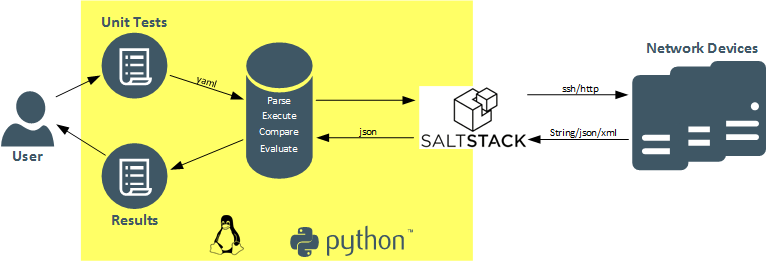
\includegraphics[width=1.00\textwidth]{./pictures/systemuebersicht.png} \\

\noindent Die zurückgegebenen Werte von SaltStack können nun mit den vom User getroffenen Annahmen verglichen und ausgewertet werden. Es kann nun festgestellt werden ob der Test bestanden wurde oder fehlgeschlagen ist. 
\newpage
\section{Klassenstruktur}
\subsection{Klassendiagramm}
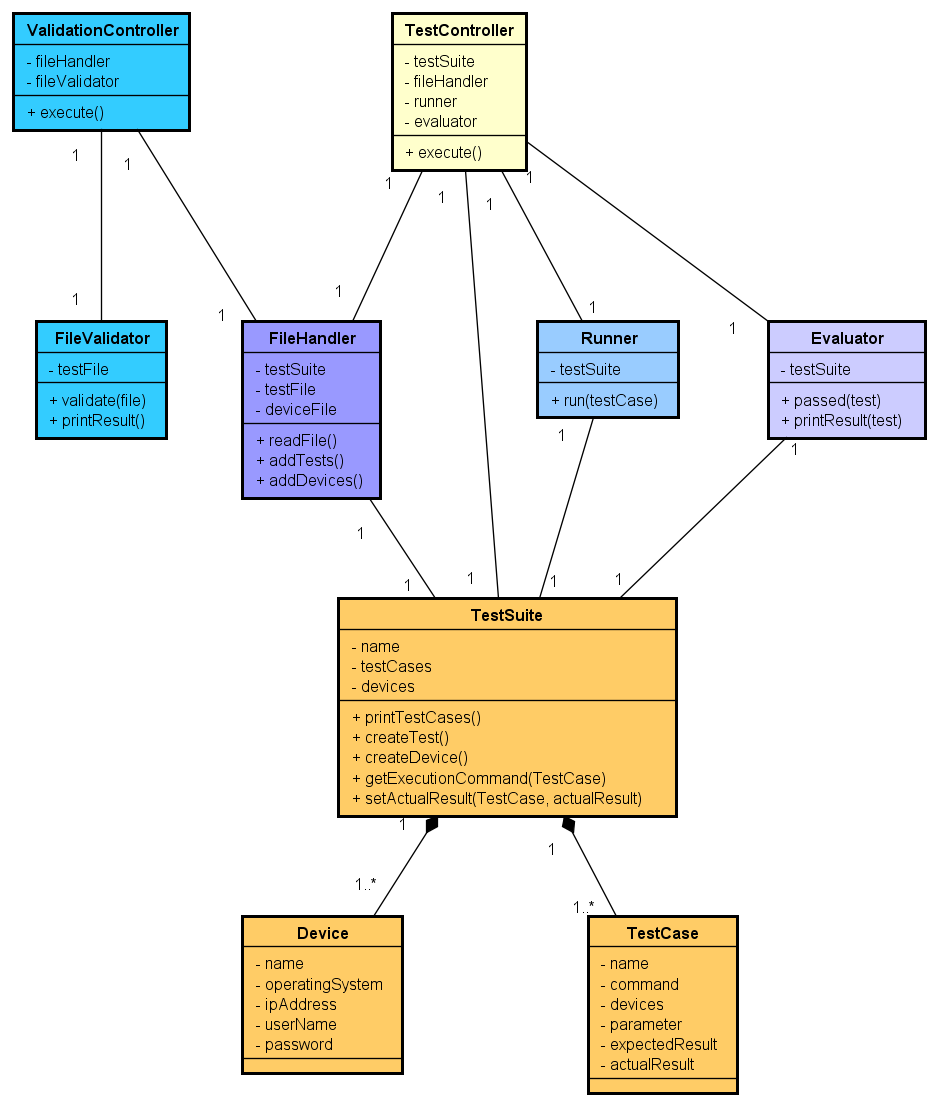
\includegraphics[width=1.02\textwidth]{./pictures/classdiagram.png}
\subsection{Klassenbeschreibungen}
\minisec{TestController}
Der TestController wird von der Main Methode gestartet, sofern die vorgesehenen Parameter mitgegeben wurden. Der TestController erzeugt im Konstruktor die benötigten Objekte und speichert sie als Referenz ab. Diese Klasse übernimmt die Steuerung und den Ablauf für die Erstellung, Durchführung und Überprüfung der Tests
\noindent \begin{table}[H]
\centering
    \begin{tabular}{@{}l p{12cm} @{}}\toprule    
    {Eigenschaft} & {Beschreibung}\\ \midrule
    testSuite & Referenz auf das TestSuite Objekt  \\       
    fileHandler & Referenz auf das FileHandler Objekt \\
    runner & Referenz auf das Runner Objekt\\
    evaluator & Referenz auf das Evaluator Objekt\\
    execute() & Methode, welche sämtlichen Operationen in der richtigen Reihenfolge auf die referenzierten Objekte durchführt\\
    \bottomrule
    \end{tabular}
\end{table}

\minisec{ValidationController}
Der ValidationController wird von der Main Methode gestartet, sofern die vorgesehenen Parameter mitgegeben wurden. Der TestController erzeugt im Konstruktor die benötigten Objekte und speichert sie als Referenz ab. Diese Klasse übernimmt die Steuerung und den Ablauf für die Erstellung, Durchführung und Validierung des TestFiles.
\noindent \begin{table}[H]
\centering
    \begin{tabular}{@{}l p{12cm} @{}}\toprule    
    {Eigenschaft} & {Beschreibung}\\ \midrule      
    fileHandler & Referenz auf das FileHandler Objekt \\
    fileValidator & Referenz auf das FileValidator Objekt\\
    execute() & Methode, welche sämtlichen Operationen in der richtigen Reihenfolge auf die referenzierten Objekte durchführt\\
    \bottomrule
    \end{tabular}
\end{table}
\newpage
\minisec{FileValidator}
Der FileValidator validiert das mitgegebene YAML Testfile auf Gültigkeit.
\noindent \begin{table}[H]
\centering
    \begin{tabular}{@{}l p{12cm} @{}}\toprule    
    {Eigenschaft} & {Beschreibung}\\ \midrule      
    testFile & YAML Testfile als Dictionary \\
    validate() & Validiert das mitgelieferte YAML File\\
    printResult() & Gibt das Resultat der Validierung aus\\
    \bottomrule
    \end{tabular}
\end{table}

\minisec{FileHandler}
der FileHandler wird vom TestController erzeugt und erhält das TestSuite Objekt von diesem. Diese Klasse liest die YAML Files ein, speichert sie in ein Dictionary.
\noindent \begin{table}[H]
\centering
    \begin{tabular}{@{}l p{12cm} @{}}\toprule    
    {Eigenschaft} & {Beschreibung}\\ \midrule
    testSuite & Referenz auf das TestSuite Objekt  \\
    testFile & Dictionary Repräsentation des YAML Test Files\\
    deviceFile & Dictionary Repräsentation des YAML Device Files\\    
    readFile() & Liest vom User mitgegebenes File ein und speichert es in die Filevariable \\
    addTests() & Iteriert durch das testFile Dictionary und erstellt Tests auf dem testSuite Objekt \\
    addDevices() & Iteriert durch das deviceFile Dictionary und erstellt Devices auf dem testSuite Objekt\\
    \bottomrule
    \end{tabular}
\end{table}

\minisec{Runner}
Die Runner Klasse führt die TestCases der TestSuite auf SaltStack aus.
\noindent \begin{table}[H]
\centering
    \begin{tabular}{@{}l p{12cm} @{}}\toprule    
    {Eigenschaft} & {Beschreibung}\\ \midrule      
    testSuite & Referenz auf das TestSuite Objekt \\
    run() & Führt die Tests der testSuite über SaltStack aus\\
    \bottomrule
    \end{tabular}
\end{table}
\newpage

\minisec{Evaluator}
Die Evaluator Klasse vergleicht Annahmen und erzielte Resultate der Tests und wertet/gibt diese aus.
\noindent \begin{table}[H]
\centering
    \begin{tabular}{@{}l p{12cm} @{}}\toprule    
    {Eigenschaft} & {Beschreibung}\\ \midrule      
    testSuite & Referenz auf das TestSuite Objekt \\
    passed() & Überprüft Annahme und erzieltes Resultat von Tests\\
    printResult() & Gibt das Ergebnis des Tests aus
    \bottomrule
    \end{tabular}
\end{table}

\minisec{TestSuite}
Die TestSuite Klasse beinhaltet sämtliche TestCases und die verwendeten Devices.
\noindent \begin{table}[H]
\centering
    \begin{tabular}{@{}l p{12cm} @{}}\toprule    
    {Eigenschaft} & {Beschreibung}\\ \midrule      
    name & Name für die TestSuite \\
    testCases & Liste von TestCase Objekten\\
    devices & Liste von Device Objekten\\
    printAllTestCases() & Gibt alle TestCases der TestSuite aus\\
    createTestCase() & Erzeugt ein TestCase Objekt und fügt es der TestSuite hinzu\\
    createDevice() & Erzeugt ein Device Objekt und fügt es der TestSuite hinzu\\
    getExecutionCommand() & Formt ein für SaltStack ausführbares Kommando eines TestCases und gibt dieses zurück\\
    setActualResult() & Setzt ein erzieltes Resultat auf einem TestCase\\
    \bottomrule
    \end{tabular}
\end{table}

\minisec{Device}
Die Device Klasse beinhaltet sämtliche Informationen eines Devices.
\noindent \begin{table}[H]
\centering
    \begin{tabular}{@{}l p{12cm} @{}}\toprule    
    {Eigenschaft} & {Beschreibung}\\ \midrule      
    name & Name für das Device \\
    operatingSystem & Angabe des zugrundeliegenden Betriebssystems\\
    ipAddress & IP Adresse des Devices\\
    userName & Username fürs Login\\
    password & Passwort fürs Login\\
    \bottomrule
    \end{tabular}
\end{table}
\minisec{TestCase}
Die Device Klasse beinhaltet sämtliche Informationen eines Devices.
\noindent \begin{table}[H]
\centering
    \begin{tabular}{@{}l p{12cm} @{}}\toprule    
    {Eigenschaft} & {Beschreibung}\\ \midrule      
    name & Name für den TestCase \\
    command & Das zu verwendende Kommando im SaltStack Modul\\
    devices & Verwendetes Device\\
    parameter & Zusatzparameter\\
    expectedResult & Resultatannahme des Users\\
    actualResult & Erzieltes Resultat des TestCases\\
    print() & Gibt den aktuellen TestCase aus\\
    \bottomrule
    \end{tabular}
\end{table}
\newpage
\section{Logische Architektur}
\begin{figure} [H]
	\begin{center}
	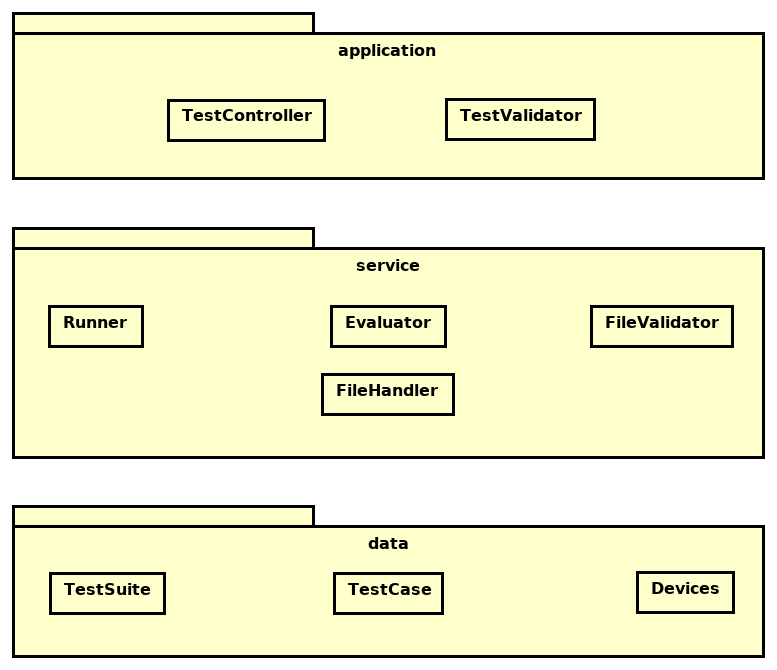
\includegraphics[width=0.90\textwidth]{./pictures/architektur.png}
	\label{Bild Referenz}
	\end{center}
\end{figure}
\begin{figure} [H]
	\begin{center}
	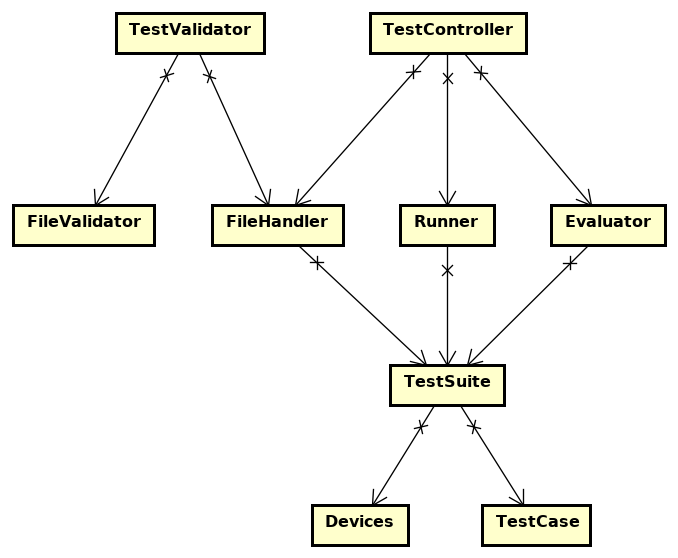
\includegraphics[width=0.90\textwidth]{./pictures/dependence_diagram.png}
	\label{Bild Referenz}
	\end{center}
\end{figure}


\subsection{Application-Layer}
Im Application-Layer befinden sich alle Abläufe, um durch das Programm zu führen. Das heisst, dass jeder Parameter seine eigene Controller-Klasse erhalten wird. Da momentan nur zwei Parameter (-i und -v) vorhanden sind, gibt es auch nur zwei Controller.
\subsubsection{Klassenstruktur}
\begin{table}[H]
\centering
    \begin{tabular}{@{}l p{11cm} @{}}\toprule    
    {Klassenname} & {Beschreibung}\\ \midrule
    ValidatorController & Der ValidatorController beinhaltet die Logik und Ausgaben, um durch die Validierung einer Datei zu führen.\\       
    TestController & Der TestController beinhaltet die gesamte Logik um Tests zu erstellen, auszuführen und zu testen. Dazu verwendet er Teile aus dem Service-Layer. \\
    \bottomrule
    \end{tabular}
\end{table}
\subsubsection{Schnittstellen}
Der Application-Layer hat momentan nur eine Schnittstelle in den Service-Layer. So kann er die verschiedenen Aufgaben an die untere schickt weiterleiten.



\subsection{Service-Layer}
Der Service-Layer beinhaltete die gesamte Programmlogik. Das heisst es gibt vier verschiedene Klassen, - Runner, FileHandler, Evaluator, FileValidator - welche jeweils ein Teil der gesamten Aufgabe übernehmen.
\subsubsection{Klassenstruktur}
\begin{table}[H]
\centering
    \begin{tabular}{@{}l p{11cm} @{}}\toprule    
    {Klassenname} & {Beschreibung}\\ \midrule
    
    Runner & Alle erfassten Tests werden durch den Runner von der TestSuite geholt und es wird ein CMD für Salt zusammengestellt. Dieses wird dann ausgeführt und die Testresultate werden der TestSuite zurückgegeben.  \\       
    Evaluator & Der Evaluator vergleicht die erwarteten Werte aus der TestSuite mit den tatsächlichen Resultaten. \\
    FileHandler & Mit dem FileHandler werden die Testfiles und die Inventoryfiles eingelesen und in Objekte umgewandelt.\\
    FileValidator & Der FileValidator überprüft ein Testfile und gibt zurück, ob dieses korrekt formatiert ist und ob die eingegebenen Parameter gültig sind. \\

    \bottomrule
    \end{tabular}
\end{table}
\subsubsection{Schnittstellen}
Der Service-Layer hat eine Schnittstelle zum Data-Layer. Durch den Service-Layer werden die Datenobjekte erstellt, bearbeitet und ausgewertet. Obere schickten müssen so immer über den Service-Layer, um eine saubere Abtrennung der Schichten zu gewährleisten.



\subsection{Data-Layer}
Der Data-Layer beinhaltet alle Datenobjekte, welche vom laufenden Programm benötigt werden.
\subsubsection{Klassenstruktur}
\begin{table}[H]
\centering
    \begin{tabular}{@{}l p{11cm} @{}}\toprule    
    {Klassenname} & {Beschreibung}\\ \midrule
    
    Testsuite & Die Testsuite beinhaltet die Logik, um neue Testcases und Devices anzulegen und abfragen auf die Daten zu machen.\\     
    TestCase & In der Klasse TestCase, werden alle Daten zu einem TestCase gespeichert. Diese kommen vom Testfile, welches der User vorgängig erfasst hat.\\         
    Devices & Alle Daten zu den einzelnen Devices aus dem Inventoryfile, werden hier als Objekt abgespeichert.\\
  
    \bottomrule
    \end{tabular}
\end{table}
\subsubsection{Schnittstellen}
Da der Data-Layer der unterste Layer ist, gibt es hier keine weiteren Schnittstellen.
\newpage
\section{Deployment Diagramm}
Hier sieht man das Deployment Diagramm mit all den wichtigen Komponenten. Man sieht wo sich Nuts befindet und wo das Modul implementiert wird.
\begin{figure} [H]
	\begin{center}
	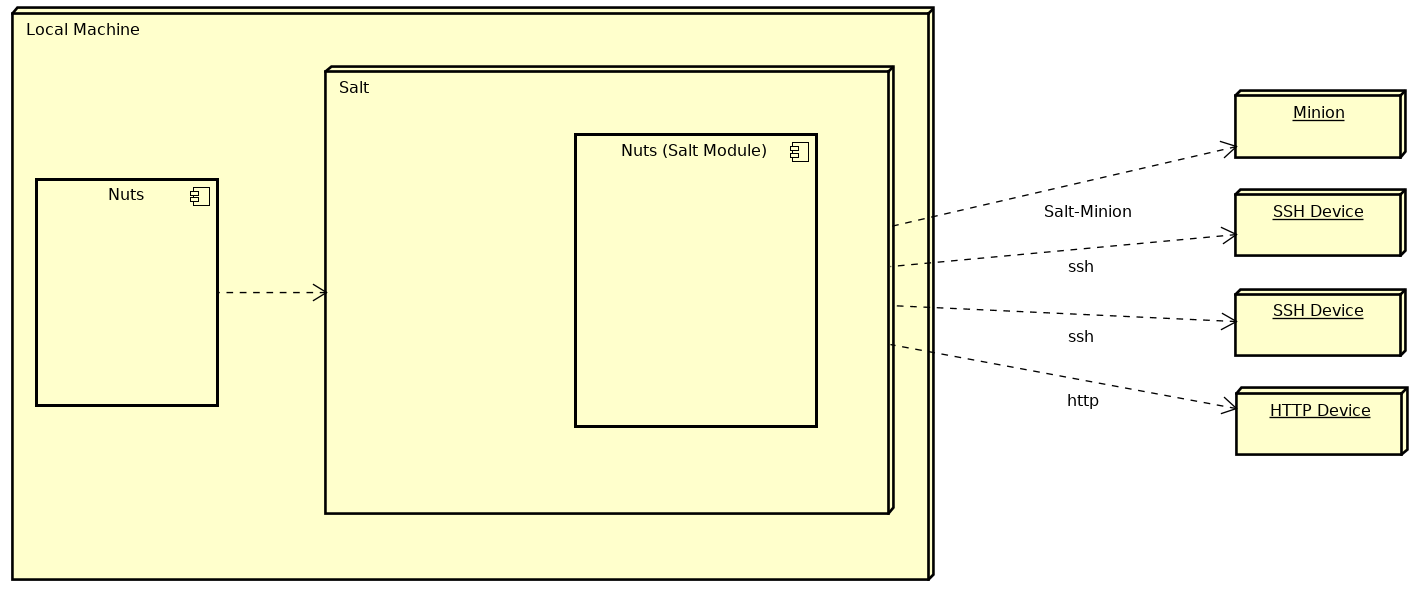
\includegraphics[width=1\textwidth]{./pictures/DeploymentDiagram.png}
	\label{Bild Referenz}
	\end{center}
\end{figure}
\newpage
\section{Sequenzdiagramm}
\begin{figure} [H]
	\begin{center}
	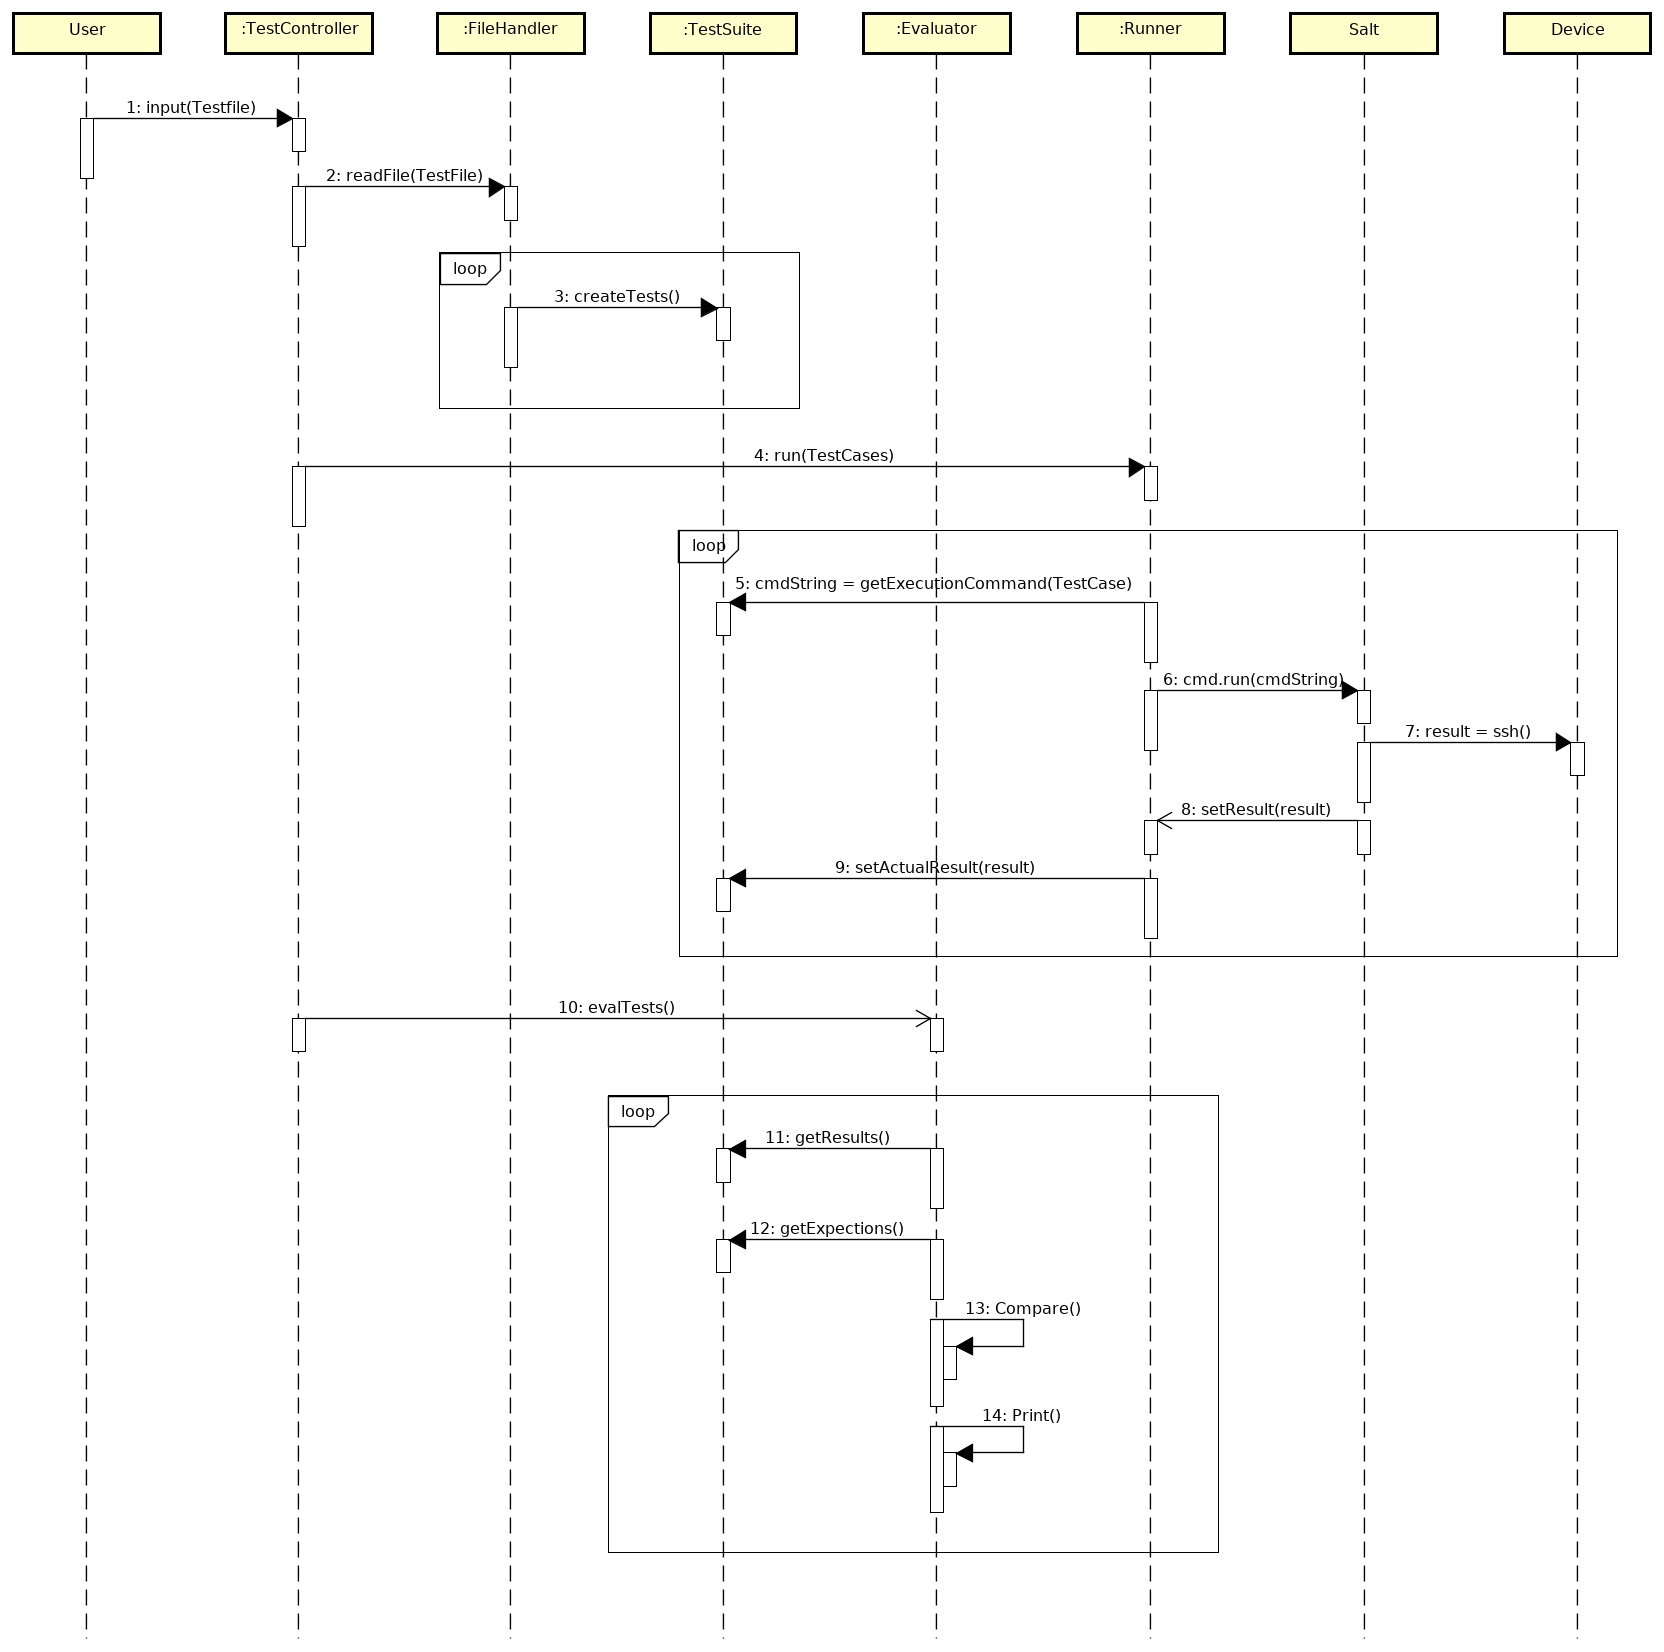
\includegraphics[width=1\textwidth]{./pictures/SequenceDiagram.png}
	\label{Bild Referenz}
	\end{center}
\end{figure}
\newpage
\section{Datensicherung}
Nuts speichert nur sehr wenige Daten. Dazu gehört ein Result-Log pro Ausführung und ein Error-Log für die Fehler.
\subsection{Testdateien}
Die erstellten Testdateien müssen von jedem Benutzer selber abgespeichert und verwaltet werden. Nuts speichert diese selber nicht ab.
\subsection{Auswertungen}
Jeder ausgeführte Test ergibt eine Log-Datei. Dieser Testlog wird unter /var/log/nuts/ gespeichert. Die Datei beinhaltet die Testergebnisse und weitere Details, falls der Test nicht bestanden ist.
\subsection{Error-Log}
Falls es beim ausführen des Programms zu einem Fehler kommt, wird dieser Fehler im Error-Log erfasst. Der Error-Log wird unter /var/log/nuts/error.log abgespeichert.

\end{document}

